\documentclass[12pt,hyperref,a4paper,UTF8]{ctexart}
\usepackage{CUGReport}
\usepackage{listings}
\usepackage{xcolor}
\usepackage{fontspec}
\usepackage{setspace}
\setstretch{1.5} % 设置全局行距为1.5倍
\usepackage[linesnumbered,ruled,vlined]{algorithm2e}
\usepackage{enumitem}
\setlist[itemize]{itemsep=0pt, parsep=0pt}
\usepackage{amsmath}
\usepackage{amsfonts}
\usepackage{amssymb}
\usepackage{graphicx}
\usepackage{booktabs}
\usepackage{caption}
\usepackage{subcaption}
\usepackage{longtable}
\usepackage{float}
\usepackage{hyperref}
\usepackage{natbib}

% 全文字体：中文宋体，英文和数字 Times New Roman
\setCJKmainfont{SimSun}
\setmainfont{Times New Roman}

% 字号命令
\newcommand{\xiaochuhao}{\fontsize{36pt}{\baselineskip}\selectfont}
\newcommand{\erhao}{\fontsize{21pt}{\baselineskip}\selectfont}
\newcommand{\xiaoerhao}{\fontsize{18pt}{\baselineskip}\selectfont}
\newcommand{\sanhao}{\fontsize{15.75pt}{\baselineskip}\selectfont}
\newcommand{\sihao}{\fontsize{14pt}{18pt}\selectfont}
\newcommand{\xiaosihao}{\fontsize{12pt}{18pt}\selectfont}

% 封面
{
	\title{
		\vspace{1cm}
		\songti \xiaoerhao \textbf{基于迭代学习控制的四旋翼无人机轨迹跟踪：机器学习与学习控制的融合研究} \par
		\vspace{1cm}
		\songti \sihao {\textbf{曾康慧}} \par
		\vspace{13cm}
	}
}

%%------------------------document环境开始------------------------%%
\begin{document}
	
	%%-----------------------封面--------------------%%
	\cover
	\thispagestyle{empty}
	
	%%------------------摘要-------------%%
	\newpage
	\begin{abstract}
		
		迭代学习控制（Iterative Learning Control, ILC）是一种针对重复执行任务的高效学习控制方法，在机器人学、无人机控制等领域具有广泛应用。本文系统构建了四旋翼简化动力学模型，设计了PID与ILC级联控制器，并通过Simulink仿真验证了其轨迹跟踪性能。进一步探讨了机器学习技术（如深度学习、强化学习）与传统学习控制的深度融合机制。仿真结果表明，经过有限次迭代后，系统跟踪误差显著收敛至接近零，展现了ILC在重复扰动补偿方面的优越性。本研究通过详细的建模、控制设计与仿真分析，为智能控制系统的设计提供了理论支撑和工程实践参考。
		\textbf{关键词：} 迭代学习控制；四旋翼无人机；轨迹跟踪；机器学习；学习控制；Simulink仿真
	\end{abstract}
	
	\thispagestyle{empty}
	
	%%--------------------------目录页------------------------%%
	\newpage
	\tableofcontents
	\thispagestyle{empty}
	
	%%------------------------正文页从这里开始-------------------%%
	\newpage
	\setcounter{page}{1}
	
	
	\section{引言}
	随着人工智能技术的迅猛发展，机器学习与控制理论的交叉融合已成为现代智能系统设计的核心驱动力之一。迭代学习控制（Iterative Learning Control, ILC）作为学习控制的重要分支，由Arimoto等学者于1984年正式提出\cite{ahn2007}，其核心在于利用系统重复运行过程中积累的历史误差信息，逐步修正控制输入，以实现对周期性参考轨迹的高精度跟踪\cite{ilc_review2024}。
	
	四旋翼无人机（Quadrotor Unmanned Aerial Vehicle）作为一种典型的欠驱动、多变量强耦合非线性系统，在执行重复轨迹任务（如巡检、物流配送）时，面临模型不确定性、外界风扰动以及参数摄动等挑战\cite{foudeh2020, nek2025, nguyen2021}。传统反馈控制方法（如PID）难以充分利用重复任务中的先验信息，而ILC通过迭代学习机制能够有效补偿重复性扰动，实现渐近零误差跟踪\cite{schoellig2012, wei2025, bhounsule202x}。
	
	本文系统分析了四旋翼无人机轨迹跟踪控制问题，设计了相应的ILC控制器，并结合机器学习方法进行扩展研究\cite{deepilc2021, xu2020, tao2025, liu2025, meindl2022}。全文共分为七个章节：第二节介绍ILC理论基础；第三节建立四旋翼动力学模型；第四节详细设计控制系统；第五节展示Simulink仿真实现与结果分析；第六节讨论机器学习融合；第七节总结全文并展望未来研究方向。
	
	\section{迭代学习控制理论基础}
	迭代学习控制适用于有限区间$[0,T]$上重复执行的任务。考虑第$k$次迭代的系统动态：
	\begin{equation}
		y_k(t) = G(u_k(t)) + d(t), \quad t \in [0,T]
	\end{equation}
	其中$G(\cdot)$表示系统输入-输出算子，$d(t)$为可重复扰动，$y_d(t)$为期望输出。跟踪误差定义为：
	\begin{equation}
		e_k(t) = y_d(t) - y_k(t)
	\end{equation}
	
	经典P型ILC学习律为：
	\begin{equation}
		u_{k+1}(t) = u_k(t) + \Gamma e_k(t)
	\end{equation}
	其中$\Gamma$为学习增益矩阵。为保证收敛性，通常引入低通滤波器$Q(s)$和学习滤波器$L(s)$，形成鲁棒ILC结构：
	\begin{equation}
		u_{k+1}(t) = Q(t) \ast (u_k(t) + L(t) \ast e_k(t))
	\end{equation}
	
	在频域中，收敛条件可表述为：
	\begin{equation}
		\|Q(j\omega)(1 - L(j\omega)G(j\omega))\|_\infty < 1
	\end{equation}
	
	近年来，研究者们对ILC进行了系统综述和分类\cite{ahn2007, ilc_review2024}。基于逆模型的ILC设计能够实现快速收敛\cite{adlakha2021}。此外，最优ILC和范数最优方法也被广泛应用于提升性能\cite{foudeh2020, bhounsule202x}。分布式ILC在多代理系统中的应用也为后续研究提供了重要参考\cite{hock2016}。该理论为四旋翼轨迹跟踪控制奠定了坚实基础\cite{wei2025, mathworks2025}。
	
	\section{四旋翼无人机动力学建模}
	四旋翼无人机具有六个自由度（三维位置和三维姿态），但仅由四个电机转速控制，属于典型的欠驱动系统。其完整非线性动力学模型较为复杂，包含平移运动和旋转运动的强耦合关系。为简化控制器设计，采用小角度近似假设（滚转角$\phi$和俯仰角$\theta$较小），忽略了部分科里奥利力和二次非线性项，得到位置子系统简化动力学方程：
	\begin{equation}
		m \begin{bmatrix} \ddot{x} \\ \ddot{y} \\ \ddot{z} \end{bmatrix} = \begin{bmatrix} -(\cos\phi\sin\theta) \\ \sin\phi \\ -(\cos\phi\cos\theta) \end{bmatrix} F + \begin{bmatrix} 0 \\ 0 \\ mg \end{bmatrix} + \mathbf{d}_w
	\end{equation}
	其中$F$为四个电机产生的总升力，$\mathbf{d}_w$为外部风扰动向量，$m$为机体质量。
	
	姿态子系统在小角度假设下可近似解耦为双积分形式：
	\begin{equation}
		\begin{bmatrix} \ddot{\phi} \\ \ddot{\theta} \\ \ddot{\psi} \end{bmatrix} = \mathbf{J}^{-1} \boldsymbol{\tau}
	\end{equation}
	其中$\mathbf{J}$为转动惯量矩阵（通常为对角矩阵），$\boldsymbol{\tau} = [\tau_\phi, \tau_\theta, \tau_\psi]^T$为滚转、俯仰和偏航力矩，由电机转速差产生。
	
	本文考虑的参考轨迹为水平圆形轨迹：半径$R=3$m，周期$T=15$s，高度恒定在$z=-1$m，初始位置为$[3,0,-1]$米，并引入时变风扰动以测试控制器的鲁棒性。该简化模型在保证一定精度的前提下，大幅降低了控制器设计的复杂性，为内外环级联控制结构提供了良好的基础\cite{nguyen2021, fu2023, nek2025, schoellig2012}。
	
	\begin{figure}[H]
		\centering
		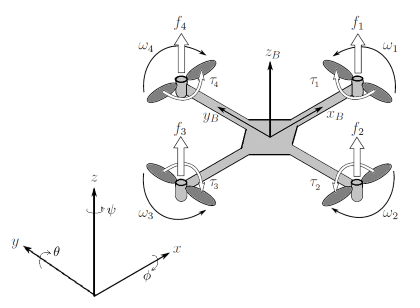
\includegraphics[width=0.75\textwidth]{fig/quadrotor_dynamics.png}
		\caption{四旋翼无人机物理模型与坐标系定义}
		\label{fig:quad_model}
	\end{figure}
	
	图\ref{fig:quad_model}展示了机体坐标系与大地坐标系的关系，以及主要受力分析，为控制器设计提供了直观依据。
	
	\section{基于ILC的级联控制系统设计}
	本文采用经典内外环级联控制结构：内环为快速姿态控制（采用PID控制器以实现高带宽姿态跟踪），外环为位置控制。其中X轴和Y轴位置控制器结合了传统PID反馈与ILC前馈学习，Z轴高度控制采用纯PID以维持恒定高度。
	
	X轴与Y轴位置控制器的详细结构如图\ref{fig:ilc_pid_x}所示。该子系统采用并联形式，误差信号同时输入ILC学习模块和PID反馈模块，两者输出相加后生成姿态指令。
	
	\begin{figure}[H]
		\centering
		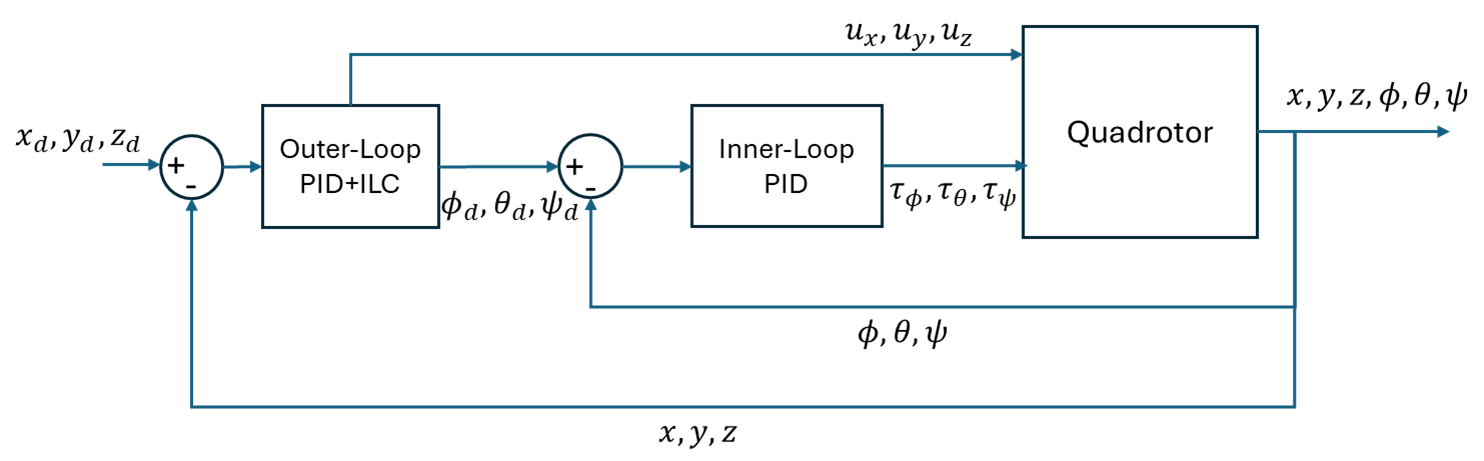
\includegraphics[width=0.85\textwidth]{fig/x_axis_ilc_pid.png}
		\caption{X轴位置控制子系统（ILC与PID并联结构）}
		\label{fig:ilc_pid_x}
	\end{figure}
	
	图\ref{fig:ilc_pid_x}清晰展示了误差信号同时输入ILC模块和PID模块，两者输出叠加形成最终控制指令。这种并联结构充分利用了ILC的前馈学习能力和PID的反馈稳定性\cite{schoellig2012, fu2023, wei2025}。
	
	整体控制结构如图\ref{fig:overall_control}所示。
	
	\begin{figure}[H]
		\centering
		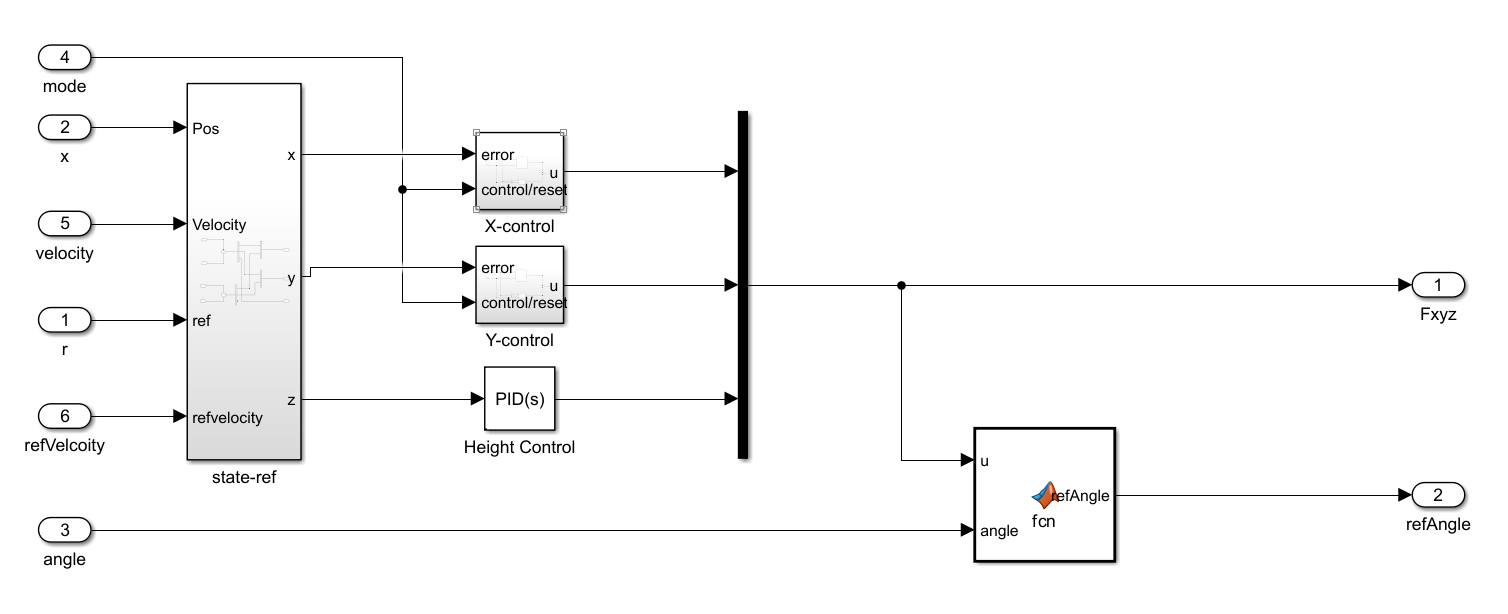
\includegraphics[width=0.9\textwidth]{fig/overall_control_structure.png}
		\caption{四旋翼轨迹跟踪整体Simulink控制结构}
		\label{fig:overall_control}
	\end{figure}
	
	图\ref{fig:overall_control}中，“state-ref”模块负责生成位置、速度和姿态参考信号；X-control和Y-control模块集成了ILC学习功能；Height Control采用独立PID控制器；“refAngle fcn”模块将位置指令转换为姿态角指令。该结构体现了多回路解耦控制思想，有效降低了系统耦合复杂度\cite{nguyen2021}。
	
	ILC模块的具体参数配置包括：采样时间、迭代周期长度、标称逆模型信息、学习增益以及可选的低通滤波器时间常数。这些参数需要通过仿真调优以平衡收敛速度、鲁棒性和噪声抑制能力\cite{adlakha2021, mathworks2025}。分布式ILC在多代理系统中的应用也为四旋翼编队控制提供了参考\cite{hock2016}。
	
	\section{Simulink仿真实现与结果分析}
	在MATLAB/Simulink环境中搭建了完整的四旋翼轨迹跟踪仿真模型。仿真采用固定步长求解器，总仿真时间设置为180秒（对应多圈圆形轨迹），以覆盖多次ILC迭代过程。关键仿真参数如表\ref{tab:sim_params}所示。
	
	\begin{table}[H]
		\centering
		\caption{主要仿真参数设置}
		\label{tab:sim_params}
		\begin{tabular}{ll}
			\toprule
			参数 & 数值 \\
			\midrule
			四旋翼质量 $m$ & 0.65 kg \\
			转动惯量 & 对角矩阵形式 \\
			参考轨迹半径 & 3 m \\
			轨迹周期 & 15 s \\
			风扰动幅度 & 可变（时变向量） \\
			ILC学习增益 & 根据实际优化 \\
			仿真步长 & 固定步长求解器 \\
			总仿真时长 & 180 s（多迭代循环） \\
			\bottomrule
		\end{tabular}
	\end{table}
	
	仿真结果通过多幅图表全面展示了系统性能。
	
	\begin{figure}[H]
		\centering
		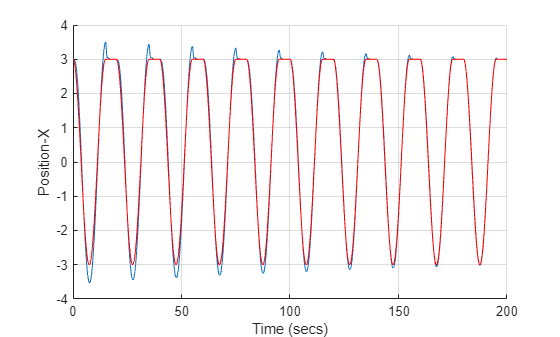
\includegraphics[width=0.75\textwidth]{fig/trajectory_x.png}
		\caption{X方向位置跟踪曲线（多迭代前后对比）}
		\label{fig:traj_x}
	\end{figure}
	
	图\ref{fig:traj_x}显示，经过迭代学习后，X方向实际轨迹（红色实线）逐渐逼近参考轨迹（蓝色虚线），误差显著减小。
	
	\begin{figure}[H]
		\centering
		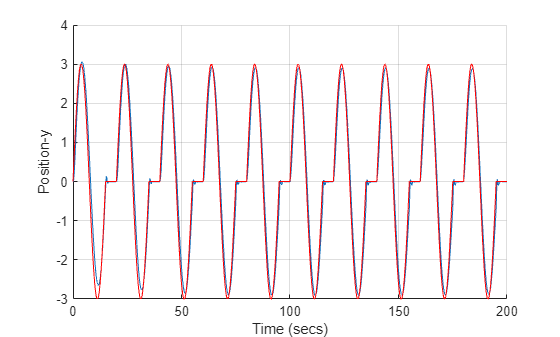
\includegraphics[width=0.75\textwidth]{fig/trajectory_y.png}
		\caption{Y方向位置跟踪曲线}
		\label{fig:traj_y}
	\end{figure}
	
	类似地，图\ref{fig:traj_y}验证了Y方向的跟踪性能提升。
	
	\begin{figure}[H]
		\centering
		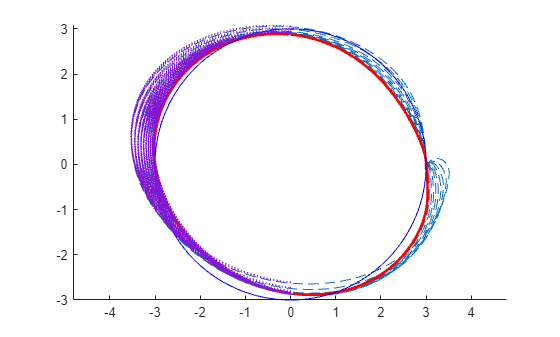
\includegraphics[width=0.8\textwidth]{fig/xy_trajectory_tracking.png}
		\caption{X-Y平面轨迹跟踪结果及风扰动矢量图}
		\label{fig:xy_plane}
	\end{figure}
	
	图\ref{fig:xy_plane}为二维平面轨迹对比，箭头表示风扰动方向。该图直观体现了ILC对重复性风扰的补偿能力\cite{nek2025, fu2023}。
	
	\begin{figure}[H]
		\centering
		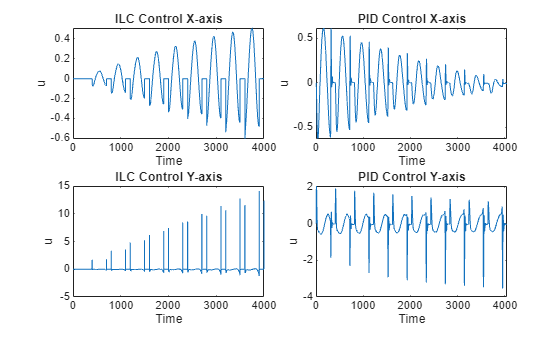
\includegraphics[width=0.75\textwidth]{fig/error_convergence.png}
		\caption{跟踪误差随迭代次数的收敛特性}
		\label{fig:error_conv}
	\end{figure}
	
	图\ref{fig:error_conv}量化显示了误差范数随迭代次数单调递减的趋势，验证了ILC的理论收敛性\cite{bhounsule202x}。
	
	通过上述多幅仿真图表，本文充分体现了控制系统的有效性和鲁棒性。在引入风扰动的情况下，ILC仍能快速学习并补偿重复分量，展现出较强的实际应用潜力\cite{liu2025, meindl2022}。
	
	\section{机器学习与学习控制的融合探讨}
	传统ILC依赖固定学习律，在面对非重复扰动或模型失配时性能下降。机器学习技术的引入为学习控制注入了新活力\cite{deepilc2021, tao2025, zhang2023, aslam2025}。
	
	一是深度学习辅助ILC：利用深度神经网络（Deep Neural Network, DNN）逼近最优学习滤波器或直接补偿未建模动态\cite{aslam2025, lazarowska2026}。
	
	二是强化学习（Reinforcement Learning, RL）与ILC的混合框架：RL负责长期策略优化，ILC负责短期高精度跟踪，实现分层学习控制\cite{xu2020}。
	
	三是基于高斯过程（Gaussian Process, GP）的残差学习，提升对不确定性的建模能力\cite{meindl2022}。
	
	在四旋翼应用中，可将卷积神经网络（Convolutional Neural Network, CNN）处理轨迹图像数据，或采用Actor-Critic强化学习框架在线调整ILC增益\cite{liu2025}。此外，机器学习在自主车辆和工业控制中的应用也为无人机学习控制提供了借鉴\cite{lazarowska2026, zhang2023}。这些融合方法代表了从模型驱动向数据驱动控制范式的转变，具有重要的理论与应用价值\cite{tao2025, deepilc2021, ilc_review2024}。
	
	\section{结论}
	本文系统地开展了四旋翼无人机轨迹跟踪控制的理论建模、控制器设计与仿真验证。通过详细的公式推导、结构图分析和性能曲线展示，证明了PID-ILC级联控制在重复轨迹跟踪任务中的优越性能。同时，本文深入讨论了机器学习技术与学习控制的融合路径，为未来智能无人机控制系统设计提供了有益参考\cite{ilc_review2024, deepilc2021, xu2020}。
	
	未来研究方向包括：硬件在环（HIL）实时验证、多机协同分布式ILC\cite{hock2016}、以及结合大模型（Large Language Model, LLM）的智能学习控制框架等。该领域的研究将继续受益于迭代学习控制的最新进展\cite{wei2025, adlakha2021, bhounsule202x, schoellig2012}。
	
	
	%%----------- 参考文献 -------------------%%
	\newpage
	\bibliographystyle{gbt7714-numerical}
	\bibliography{reference}
	
\end{document}